% Options for packages loaded elsewhere
% Options for packages loaded elsewhere
\PassOptionsToPackage{unicode}{hyperref}
\PassOptionsToPackage{hyphens}{url}
\PassOptionsToPackage{dvipsnames,svgnames,x11names}{xcolor}
%
\documentclass[
  11pt,
]{article}
\usepackage{xcolor}
\usepackage[top=0.4in,bottom=0.45in,left=0.65in,right=0.65in,includehead,headheight=52pt,headsep=7pt,includefoot,footskip=24pt]{geometry}
\usepackage{amsmath,amssymb}
\setcounter{secnumdepth}{-\maxdimen} % remove section numbering
\usepackage{iftex}
\ifPDFTeX
  \usepackage[T1]{fontenc}
  \usepackage[utf8]{inputenc}
  \usepackage{textcomp} % provide euro and other symbols
\else % if luatex or xetex
  \usepackage{unicode-math} % this also loads fontspec
  \defaultfontfeatures{Scale=MatchLowercase}
  \defaultfontfeatures[\rmfamily]{Ligatures=TeX,Scale=1}
\fi
\usepackage{lmodern}
\ifPDFTeX\else
  % xetex/luatex font selection
\fi
% Use upquote if available, for straight quotes in verbatim environments
\IfFileExists{upquote.sty}{\usepackage{upquote}}{}
\IfFileExists{microtype.sty}{% use microtype if available
  \usepackage[]{microtype}
  \UseMicrotypeSet[protrusion]{basicmath} % disable protrusion for tt fonts
}{}
\makeatletter
\@ifundefined{KOMAClassName}{% if non-KOMA class
  \IfFileExists{parskip.sty}{%
    \usepackage{parskip}
  }{% else
    \setlength{\parindent}{0pt}
    \setlength{\parskip}{6pt plus 2pt minus 1pt}}
}{% if KOMA class
  \KOMAoptions{parskip=half}}
\makeatother
% Make \paragraph and \subparagraph free-standing
\makeatletter
\ifx\paragraph\undefined\else
  \let\oldparagraph\paragraph
  \renewcommand{\paragraph}{
    \@ifstar
      \xxxParagraphStar
      \xxxParagraphNoStar
  }
  \newcommand{\xxxParagraphStar}[1]{\oldparagraph*{#1}\mbox{}}
  \newcommand{\xxxParagraphNoStar}[1]{\oldparagraph{#1}\mbox{}}
\fi
\ifx\subparagraph\undefined\else
  \let\oldsubparagraph\subparagraph
  \renewcommand{\subparagraph}{
    \@ifstar
      \xxxSubParagraphStar
      \xxxSubParagraphNoStar
  }
  \newcommand{\xxxSubParagraphStar}[1]{\oldsubparagraph*{#1}\mbox{}}
  \newcommand{\xxxSubParagraphNoStar}[1]{\oldsubparagraph{#1}\mbox{}}
\fi
\makeatother


\usepackage{longtable,booktabs,array}
\newcounter{none} % for unnumbered tables
\usepackage{calc} % for calculating minipage widths
% Correct order of tables after \paragraph or \subparagraph
\usepackage{etoolbox}
\makeatletter
\patchcmd\longtable{\par}{\if@noskipsec\mbox{}\fi\par}{}{}
\makeatother
% Allow footnotes in longtable head/foot
\IfFileExists{footnotehyper.sty}{\usepackage{footnotehyper}}{\usepackage{footnote}}
\makesavenoteenv{longtable}
\usepackage{graphicx}
\makeatletter
\newsavebox\pandoc@box
\newcommand*\pandocbounded[1]{% scales image to fit in text height/width
  \sbox\pandoc@box{#1}%
  \Gscale@div\@tempa{\textheight}{\dimexpr\ht\pandoc@box+\dp\pandoc@box\relax}%
  \Gscale@div\@tempb{\linewidth}{\wd\pandoc@box}%
  \ifdim\@tempb\p@<\@tempa\p@\let\@tempa\@tempb\fi% select the smaller of both
  \ifdim\@tempa\p@<\p@\scalebox{\@tempa}{\usebox\pandoc@box}%
  \else\usebox{\pandoc@box}%
  \fi%
}
% Set default figure placement to htbp
\def\fps@figure{htbp}
\makeatother





\setlength{\emergencystretch}{3em} % prevent overfull lines

\providecommand{\tightlist}{%
  \setlength{\itemsep}{0pt}\setlength{\parskip}{0pt}}



 


% =====================================================================
%  _style.tex  ·  Design system for EIL research highlights (v4 layout)
%  Edit here to restyle ALL research highlights. Included via the .qmd YAML.
%  Matches the canonical single-column v4 template; the masthead and footer
%  are set per-document via fancyhdr in each .qmd's include-in-header.
% =====================================================================

% ---- Colours (exact hex) --------------------------------------------
\definecolor{ink}{HTML}{1D2620}        % headings, title, section heads, rule
\definecolor{body}{HTML}{33352C}       % main body paragraphs
\definecolor{accentred}{HTML}{641111}  % RESEARCH HIGHLIGHT label, links, fig title
\definecolor{boxred}{HTML}{8C2826}     % Bottom Line box fill
\definecolor{boxtext}{HTML}{EEF1EA}    % Bottom Line body text (off-white)
\definecolor{muted}{HTML}{50534A}      % figure source line
\definecolor{cite}{HTML}{6E6D61}       % citation line
\definecolor{faint}{HTML}{9A978A}      % footer
\definecolor{warmrule}{HTML}{D8D2C2}   % thin warm-grey dividers
\definecolor{paper}{HTML}{FAF8F1}      % warm page background

% \pagecolor{paper}                    % uncomment for warm off-white background

% ---- Fonts (Source Sans 3 / Source Serif 4) -------------------------
\usepackage[T1]{fontenc}
\usepackage[default]{sourcesanspro}
\usepackage{sourceserifpro}
\renewcommand{\familydefault}{\sfdefault}

% ---- Page -----------------------------------------------------------
\pagestyle{empty}
\setlength{\parindent}{0pt}
\setlength{\parskip}{2pt}
% Default body size/colour. The v4 .qmd overrides this to 10.5/13.5pt.
\AtBeginDocument{\color{body}\fontsize{9.4pt}{13.6pt}\selectfont}

% ---- Packages -------------------------------------------------------
\usepackage{microtype}
\usepackage{soul}
\setul{2pt}{.5pt}
\usepackage{tcolorbox}
\tcbuselibrary{skins}
\usepackage[colorlinks=true, urlcolor=accentred, linkcolor=accentred, pdfborder={0 0 0}]{hyperref}

% =====================================================================
%  MACROS
% =====================================================================

% --- Title + citation (citation has a thin warm divider beneath) ------
\newcommand{\brieftitle}[1]{%
  {\color{ink}\fontsize{18pt}{19.5pt}\selectfont\bfseries\textls[-12]{#1}\par}\vspace{3pt}}
\newcommand{\briefcitation}[1]{%
  {\color{cite}\fontsize{9.4pt}{12pt}\selectfont #1\par}\vspace{3pt}%
  \noindent\textcolor{warmrule}{\rule{\linewidth}{0.7pt}}}

% --- Section heads (uppercase, ink) ----------------------------------
\newcommand{\sectionhead}[1]{%
  \vspace{2pt}{\color{ink}\bfseries\fontsize{9.75pt}{12pt}\selectfont
  \textls[20]{\MakeUppercase{#1}}\par}\vspace{1pt}}

% --- Sub-heads (small uppercase) — Takeaway subheads -----------------
% The v4 .qmd overrides this to the brand maroon via \renewcommand.
\newcommand{\subhead}[1]{%
  {\color{ink}\bfseries\fontsize{8.25pt}{10pt}\selectfont
  \textls[50]{\MakeUppercase{#1}}\par}\vspace{2pt}}

% --- Figure title + source line --------------------------------------
\newcommand{\figtitle}[2]{%
  {\bfseries\color{accentred}\fontsize{7.1pt}{9pt}\selectfont\textls[40]{\MakeUppercase{#1}}}\par%
  {\color{muted}\fontsize{7.1pt}{9pt}\selectfont #2}\par\vspace{4pt}}

% =====================================================================
%  COLOURED BOXES
% =====================================================================

% --- Bottom Line box (border-radius 6px -> arc=4pt) ------------------
\newtcolorbox{bottomline}{%
  enhanced, arc=4pt, outer arc=4pt, boxrule=0pt,
  colback=boxred, coltext=boxtext,
  left=7pt, right=7pt, top=7pt, bottom=7pt,
  before upper={\fontsize{9.4pt}{13.6pt}\selectfont}}

% --- Info box (contact + full citation; centered, thin faint border) --
% Superseded by the moreinfo environment below; kept so older highlights
% still compile. Faint text at footer size. Wrap any link as
% \href{url}{\color{faint}\underline{text}} so it inherits the faint
% colour instead of the global accent link colour.
\newtcolorbox{infobox}{%
  enhanced, width=0.9\linewidth, center, arc=4pt, outer arc=4pt,
  boxrule=0.5pt, colframe=faint, colback=white, coltext=faint,
  left=9pt, right=9pt, top=7pt, bottom=7pt,
  before upper={\fontsize{7.4pt}{9.5pt}\selectfont}}

% =====================================================================
%  CLOSING BLOCK
% =====================================================================

% --- For more information (full width; rule above, no box) ------------
% Citation, author affiliations + contact, then the EIL boilerplate —
% one paragraph each. Wrap any link as
% \href{url}{\color{cite}\underline{text}} so it inherits the block's
% grey instead of the global accent link colour.
\newenvironment{moreinfo}{%
  \par\vspace{12pt}%
  \noindent\textcolor{warmrule}{\rule{\linewidth}{0.7pt}}\par
  \vspace{7pt}%
  {\color{ink}\bfseries\fontsize{8.25pt}{10pt}\selectfont
   \textls[50]{\MakeUppercase{For more information}}\par}\vspace{4pt}%
  \color{cite}\fontsize{8.4pt}{11.5pt}\selectfont
  \setlength{\parskip}{5pt}%
}{\par}
% --- Running masthead + footer (logo, label, rule, page number) ---
\usepackage{fancyhdr}
\renewcommand{\headrulewidth}{0pt}
\renewcommand{\footrulewidth}{0pt}
\fancypagestyle{brief}{%
  \fancyhf{}%
  \fancyhead[L]{%
    \begin{minipage}[c]{0.62\textwidth}\raggedright\color{ink}
\includegraphics[height=0.45in]{../../../../formats/logos/eil-logo-maroon.png}\end{minipage}\hfill%
    \begin{minipage}[c]{0.36\textwidth}\raggedleft\fontsize{8.25pt}{10pt}\selectfont\bfseries\color{accentred}\textls[200]{\MakeUppercase{Research Highlight}}\end{minipage}%
    \par\vspace{2pt}%
    \noindent\textcolor{ink}{\rule{\textwidth}{2.2pt}}%
  }%
  \fancyfoot[C]{%
    \color{warmrule}\rule{\textwidth}{0.7pt}\par\vspace{3pt}%
    \hbox to\textwidth{%
      \color{faint}\fontsize{7.4pt}{9pt}\selectfont
      For full paper:\hspace{0.4em}\href{https://doi.org/10.1002/pam.70056}{\color{faint}\underline{\textls[40]{doi.org/10.1002/pam.70056}}}%
      \hfill
      Page \thepage%
    }%
  }%
}
\pagestyle{brief}
% Subhead macro retained from the design system (unused in v5, which
% replaces the Takeaways subheads with a flowing concluding section).
\renewcommand{\subhead}[1]{%
  {\color{accentred}\bfseries\fontsize{8.25pt}{10pt}\selectfont
  \textls[50]{\MakeUppercase{#1}}\par}\vspace{2pt}}
\makeatletter
\@ifpackageloaded{caption}{}{\usepackage{caption}}
\AtBeginDocument{%
\ifdefined\contentsname
  \renewcommand*\contentsname{Table of contents}
\else
  \newcommand\contentsname{Table of contents}
\fi
\ifdefined\listfigurename
  \renewcommand*\listfigurename{List of Figures}
\else
  \newcommand\listfigurename{List of Figures}
\fi
\ifdefined\listtablename
  \renewcommand*\listtablename{List of Tables}
\else
  \newcommand\listtablename{List of Tables}
\fi
\ifdefined\figurename
  \renewcommand*\figurename{Figure}
\else
  \newcommand\figurename{Figure}
\fi
\ifdefined\tablename
  \renewcommand*\tablename{Table}
\else
  \newcommand\tablename{Table}
\fi
}
\@ifpackageloaded{float}{}{\usepackage{float}}
\floatstyle{ruled}
\@ifundefined{c@chapter}{\newfloat{codelisting}{h}{lop}}{\newfloat{codelisting}{h}{lop}[chapter]}
\floatname{codelisting}{Listing}
\newcommand*\listoflistings{\listof{codelisting}{List of Listings}}
\makeatother
\makeatletter
\makeatother
\makeatletter
\@ifpackageloaded{caption}{}{\usepackage{caption}}
\@ifpackageloaded{subcaption}{}{\usepackage{subcaption}}
\makeatother
\usepackage{bookmark}
\IfFileExists{xurl.sty}{\usepackage{xurl}}{} % add URL line breaks if available
\urlstyle{same}
\hypersetup{
  colorlinks=true,
  linkcolor={blue},
  filecolor={Maroon},
  citecolor={Blue},
  urlcolor={Blue},
  pdfcreator={LaTeX via pandoc}}


\author{}
\date{}
\begin{document}


% ---------------------------------------------------------------------
% TITLE + CITATION  (masthead repeats in the page header)
% ---------------------------------------------------------------------
\brieftitle{EPA Compliance Assistance Workshops Don't Reduce Violations}
\briefcitation{Lessons from ``The Effect of Compliance Assistance on Pollution Discharges and Violations of Environmental Regulations'' by Paul J. Ferraro \& Jay P. Shimshack in \textit{Journal of Policy Analysis and Management}, 2026.}

\vspace{-2pt}

% override body font size for this document
\fontsize{10.5pt}{13.5pt}\selectfont

% ---------------------------------------------------------------------
% BOTTOM LINE
% ---------------------------------------------------------------------
\begin{bottomline}
{\fontsize{11pt}{15pt}\selectfont
\textbf{Offering polluting facilities free help to follow the rules doesn't make them more likely to follow them.} New research studying hundreds of facilities that were offered free compliance assistance workshops found the workshops didn't reduce violations.
}
\end{bottomline}

\vspace{6pt}

% ---------------------------------------------------------------------
% BACKGROUND  (broad — poses the question)
% ---------------------------------------------------------------------
\sectionhead{Background}
\noindent Environmental enforcement in the U.S. has long centered on inspecting facilities, catching violations, and levying fines. \textbf{Compliance assistance} takes a different approach: regulators offer workshops, technical guidance, and other support to help facilities understand and meet regulatory requirements. This approach reflects the idea that many violations result from confusion or limited expertise rather than deliberate corner-cutting. Compliance assistance has become a prominent alternative to enforcement action at the Environmental Protection Agency (EPA), and was recently adopted by the Ohio EPA in a program offering free workshops to wastewater treatment facilities across the state.

\noindent \textbf{In a new study, Ferraro and Shimshack (2026) find that compliance assistance workshops did not reduce regulatory violations or pollution discharges.} The researchers analyzed data from hundreds of Ohio wastewater treatment facilities that had recently been cited for violations and were invited to attend workshops rolled out over several months. An earlier, noncausal evaluation had suggested the program was effective, based on a simple before-and-after comparison of violation rates. Such comparisons can be misleading, and accurately understanding program effects is critical to promoting environmental compliance in real-world policy settings.


\vspace{6pt}

% ---------------------------------------------------------------------
% FIGURE — event study: effect on violations by month around training
%   Placed after the background so it lands on page 1: the bottom-line box
%   has already stated the null, so the chart illustrates a claim the
%   reader holds rather than spoiling one they don't.
% ---------------------------------------------------------------------
\begin{center}
\begin{minipage}{0.75\linewidth}
\figtitle{The workshops' effect on violations, month by month}{Source: Ferraro \& Shimshack (2026), Fig.\ 2a.}
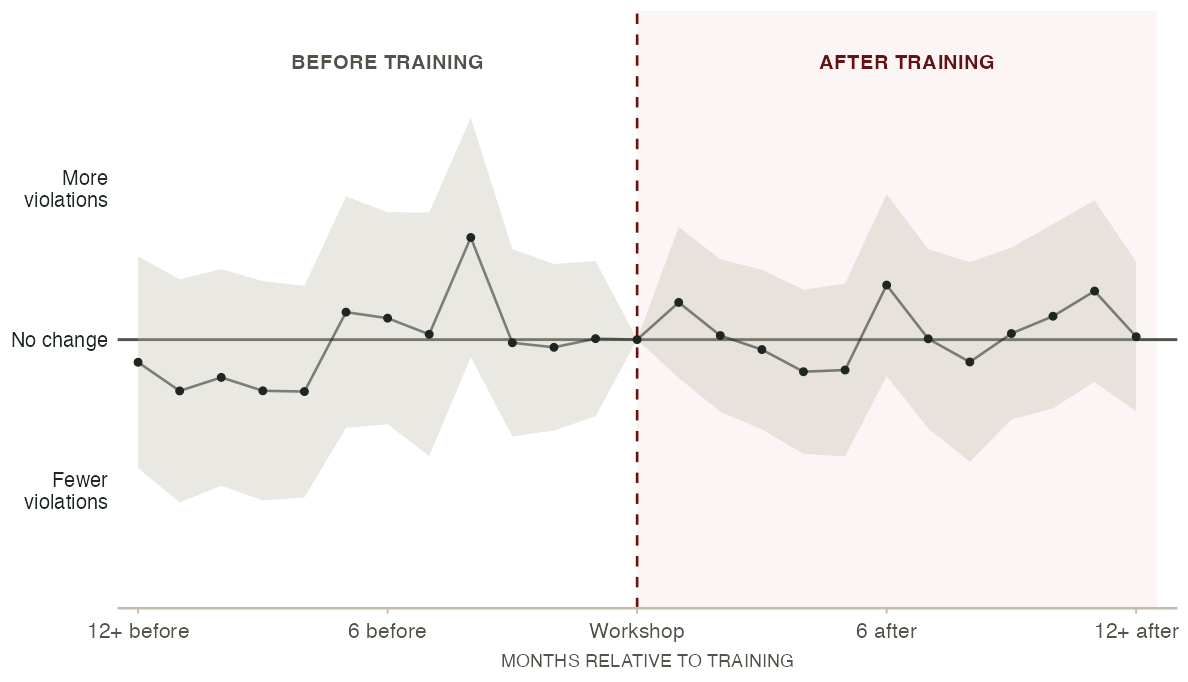
\includegraphics[width=\linewidth]{../../data-viz/figures/fig2-event-study.png}
\par\vspace{3pt}
{\color{faint}\fontsize{7.1pt}{9.5pt}\selectfont \textit{Note:} This figure shows the estimated effect of compliance assistance workshops on the number of facility violations. Each dot shows whether facilities had more (above the zero line) or fewer (below the zero line) violations in a given month relative to the workshop month (vertical dashed line). The estimates account for each facility's usual number of violations, the local weather, and any common trends shared across facilities; the shaded band shows the range of estimates within the 95\% confidence interval. If the workshops had an effect on violations, the line would drop below zero after the workshop.\par}
\end{minipage}
\end{center}

\vspace{6pt}

% ---------------------------------------------------------------------
% HOW THE STUDY TESTED IT  (narrowing — setting + research design)
% ---------------------------------------------------------------------
\sectionhead{Comparing across time and facilities}
\noindent \textbf{Measuring whether a policy works requires a comparison group: facilities that show what the trained facilities would have done without the training.} Comparing violations at trained facilities before and after the workshops would credit the training with anything else that changed over the same period. Comparing facilities that signed up against those that did not introduces a different problem: attendance was voluntary, so a gap between the two groups could reflect the motivation of the facilities that chose to participate rather than the effect of the training.

\noindent Ferraro and Shimshack addressed this by comparing facilities trained earlier against facilities that had also signed up but had not yet been trained. Both groups had volunteered, and both were tracked over the same months, so any trend running through the industry appeared in both. The staggered rollout of the workshops is what made the not-yet-trained facilities available as a benchmark. The comparison holds only if those facilities would otherwise have followed the same path as the trained ones, an assumption the pre-workshop months in the figure support but cannot prove.

\vspace{6pt}


% ---------------------------------------------------------------------
% WHAT THE STUDY FOUND  (the waist — result, precision, discharges)
% ---------------------------------------------------------------------
\sectionhead{No effect on violations or discharges}
\noindent \textbf{Trained facilities were no less likely to violate environmental regulations than facilities that had not yet been trained.} A violation is a regulatory event rather than a measure of pollution, so Ferraro and Shimshack also measured discharges directly, across five pollutants. Both sets of estimates were close to zero and precisely estimated. The workshops changed neither what facilities reported nor what they released into the water.

\noindent \textbf{Violations did fall at the facilities that attended, but the workshops were not the reason.} At those plants, violations fell by about half in the years after the training. They fell just as far at the facilities that had signed up but had not yet been trained. Looking only at the facilities that attended, the earlier before-and-after evaluation counted that decline as evidence the program worked.

\noindent Compliance assistance rests on the premise that facilities break the rules because they do not fully understand them. The results do not support that premise for these wastewater plants: if facilities were violating out of confusion, the training would have reduced violations, and it did not. \textbf{The pattern is more consistent with facilities weighing the cost of compliance against the consequences of violating.} Free help was not what these facilities were missing.

\vspace{8pt}

\begin{moreinfo}
Ferraro, Paul J., and Jay P. Shimshack. 2026. ``The Effect of Compliance Assistance on Pollution Discharges and Violations of Environmental Regulations.'' \textit{Journal of Policy Analysis and Management} 45 (3): e70056. \href{https://doi.org/10.1002/pam.70056}{\color{cite}\underline{doi.org/10.1002/pam.70056}}.\par

Paul J. Ferraro is at Johns Hopkins University. Jay P. Shimshack is at the University of Virginia. Contact Jay Shimshack (jay.shimshack@virginia.edu) with questions about this research.\par

The \href{https://www.environmental-inequality-lab.org/}{\color{cite}\underline{Environmental Inequality Lab}} is a nonpartisan research group that applies a rigorous, data-driven approach to understand how our environment shapes economic opportunity and well-being.\par
\end{moreinfo}




\end{document}
